%%%%%%%%%%%%%%%%%%%%%%% file template.tex %%%%%%%%%%%%%%%%%%%%%%%%%
%
% This is a general template file for the LaTeX package SVJour3
% for Springer journals.          Springer Heidelberg 2010/09/16
%
% Copy it to a new file with a new name and use it as the basis
% for your article. Delete % signs as needed.
%
% This template includes a few options for different layouts and
% content for various journals. Please consult a previous issue of
% your journal as needed.
%
%%%%%%%%%%%%%%%%%%%%%%%%%%%%%%%%%%%%%%%%%%%%%%%%%%%%%%%%%%%%%%%%%%%
%
% First comes an example EPS file -- just ignore it and
% proceed on the \documentclass line
% your LaTeX will extract the file if required
\begin{filecontents*}{example.eps}
%!PS-Adobe-3.0 EPSF-3.0
%%BoundingBox: 19 19 221 221
%%CreationDate: Mon Sep 29 1997
%%Creator: programmed by hand (JK)
%%EndComments
gsave
newpath
  20 20 moveto
  20 220 lineto
  220 220 lineto
  220 20 lineto
closepath
2 setlinewidth
gsave
  .4 setgray fill
grestore
stroke
grestore
\end{filecontents*}
%
\RequirePackage{fix-cm}
%
%\documentclass{svjour3}                     % onecolumn (standard format)
%\documentclass[smallcondensed]{svjour3}     % onecolumn (ditto)
\documentclass[smallextended]{svjour3}       % onecolumn (second format)
%\documentclass[twocolumn]{svjour3}          % twocolumn
%
\smartqed  % flush right qed marks, e.g. at end of proof
%
\usepackage{graphicx}
%
% \usepackage{mathptmx}      % use Times fonts if available on your TeX system
%
% insert here the call for the packages your document requires
%\usepackage{latexsym}
% etc.
%
% please place your own definitions here and don't use \def but
% \newcommand{}{}
%
% Insert the name of "your journal" with
% \journalname{myjournal}
%
\begin{document}

\title{Indirect Bibliometrics by Hypernetwork Analysis%\thanks{Grants or other notes
%about the article that should go on the front page should be
%placed here. General acknowledgments should be placed at the end of the article.}
}
%\subtitle{Do you have a subtitle?\\ If so, write it here}

%\titlerunning{Short form of title}        % if too long for running head

\author{First Author         \and
        Second Author %etc.
}

%\authorrunning{Short form of author list} % if too long for running head

\institute{F. Author \at
              first address \\
              Tel.: +123-45-678910\\
              Fax: +123-45-678910\\
              \email{fauthor@example.com}           %  \\
%             \emph{Present address:} of F. Author  %  if needed
           \and
           S. Author \at
              second address
}

\date{Received: date / Accepted: date}
% The correct dates will be entered by the editor


\maketitle

\begin{abstract}
Insert your abstract here. Include keywords, PACS and mathematical
subject classification numbers as needed.
\keywords{First keyword \and Second keyword \and More}
% \PACS{PACS code1 \and PACS code2 \and more}
% \subclass{MSC code1 \and MSC code2 \and more}
\end{abstract}

\section{Introduction}
\label{intro}


Semantic analysis does not contain all the information on disciplinary compartmentation nor on patterns of propagation of scientific knowledge as the ones contained in citation networks for example. Furthermore, data collection in the previous algorithm is subject to convergence towards self-consistent themes because of the proper structure of the method. It may give more insight about scientific social patterns of ontological choices in modeling to study communities in broader networks, that would more correspond to disciplines (or sub-disciplines depending on granularity level).

Previous works in quantitative epistemology using various types of networks have shown interesting potentialities. For the citation network, a good predicting power for citation patterns is for example obtained in~\cite{2013arXiv1310.8220N}. Co-authorship networks can also be used for predictive models~\cite{2014arXiv1402.7268S}. A multilayer network approach was recently proposed in~\cite{2016arXiv160106075O}, using bipartites networks of papers and scholars, in order to produce measures of interdisciplinarity. Disciplines can be stratified into layers to reveal communities between them and therein collaboration patterns~\cite{2015arXiv150601280B}. Keyword networks are used in other fields such as economics of technology~\cite{choi2014patent,shibata2008detecting}.

We describe here a study implementing these ideas for the particular case of a scientific journal for which bibliographical data is difficult to obtain, that is \texttt{cybergeo}, an electronic journal in theoretical and quantitative geography, that is concerned with open science issues such as peer-review ethics transparency~\cite{10.1371/journal.pone.0147913}. Our approach combine semantic communities analysis (as done in~\cite{2016arXiv160208451P} but with keyword extraction ; \cite{2015arXiv151003797G} analyses semantic networks of political debates) with citation network to extract e.g. interdisciplinarity measures.





\section{Material and Methods}
\label{sec:1}




\subsubsection{Implementation}

The general architecture for data collection is presented in Fig.~\ref{fig:quantepistemo:data}. Citation data is collected from \texttt{Google Scholar}, that is the only source for incoming citations~\cite{noruzi2005google} in our case as the journal is not referenced in other databases. We are aware of the possible biaises using this single source~\cite{bohannon2014scientific}\footnote{or see \url{http://iscpif.fr/blog/2016/02/the-strange-arithmetic-of-google-scholars/}}, but these critics are more directed towards search results than citation counts. 

Text processing is done the same way as in previous section, expect that a particular treatment is done to language detection using \emph{stop-words} and a specific tagger \texttt{TreeTagger} is used for other languages than english~\cite{schmid1994probabilistic}.


%%%%%%%%%%%%%%%%%%
\begin{figure}
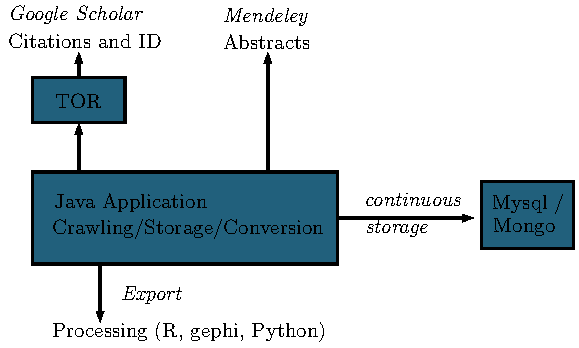
\includegraphics[width=\textwidth]{figures/archi}
\caption[Heterogeneous Bibliographical Data Collection]{Heterogeneous Bibliographical Data Collection. Architecture of the application for content (semantic data), metadata and citation data collection.}
\label{fig:datacollection}
\end{figure}
%%%%%%%%%%%%%%%%%%





%%%%%%%%%%%%%%%%%%
\section{Results}



We show in figures~\ref{fig:quantepistemo:citnw} and~\ref{fig:quantepistemo:semanticnw} preliminary results on citation and semantic network. We are able by the reconstruction of the citation network at depth $\pm 1$ from the original 1000 references of the journal to retrieve around $45\cdot 10^6$ references, on which $2.1\cdot 10^6$ are retrieved with abstract text allowing semantic analysis. We retrieve by community detection in the semantic network typical geographical disciplines, such as :

\begin{itemize}
\item Hydrology : \texttt{water, basin, river, capac}
\item Traffic : \texttt{traffic, road, vehicl}
\item Biogeography : \texttt{habitat, soil, veget, ecosystem}
\item Political Science : \texttt{polit, cultur, societi, debat}
\item Economy : \texttt{market, economi, privat, competit, industri}
\item Transportation : \texttt{transport, travel}
\item Teledetection : \texttt{cluster, imag, classif, satellit}
\item Education : \texttt{educ, age, student, school}
\item Health : \texttt{diseas, infect}
\item GIS : \texttt{gi, geograph inform system}
\item Social geography : \texttt{neighborhood, resid}
\end{itemize}



Distribution of keywords within reconstructed disciplines provides an article-level interdisciplinarity, and we can construct various measures at the journal level. Combination of citation and semantic layers in the hyper-network provide second order interdisciplinarity measures. The construction of null models for comparison and the collection of currently missing data (journals for other papers) are currently ongoing so these results are not presented here.





%%%%%%%%%%%%%%%%%
\begin{figure}
%\hspace{-3cm}
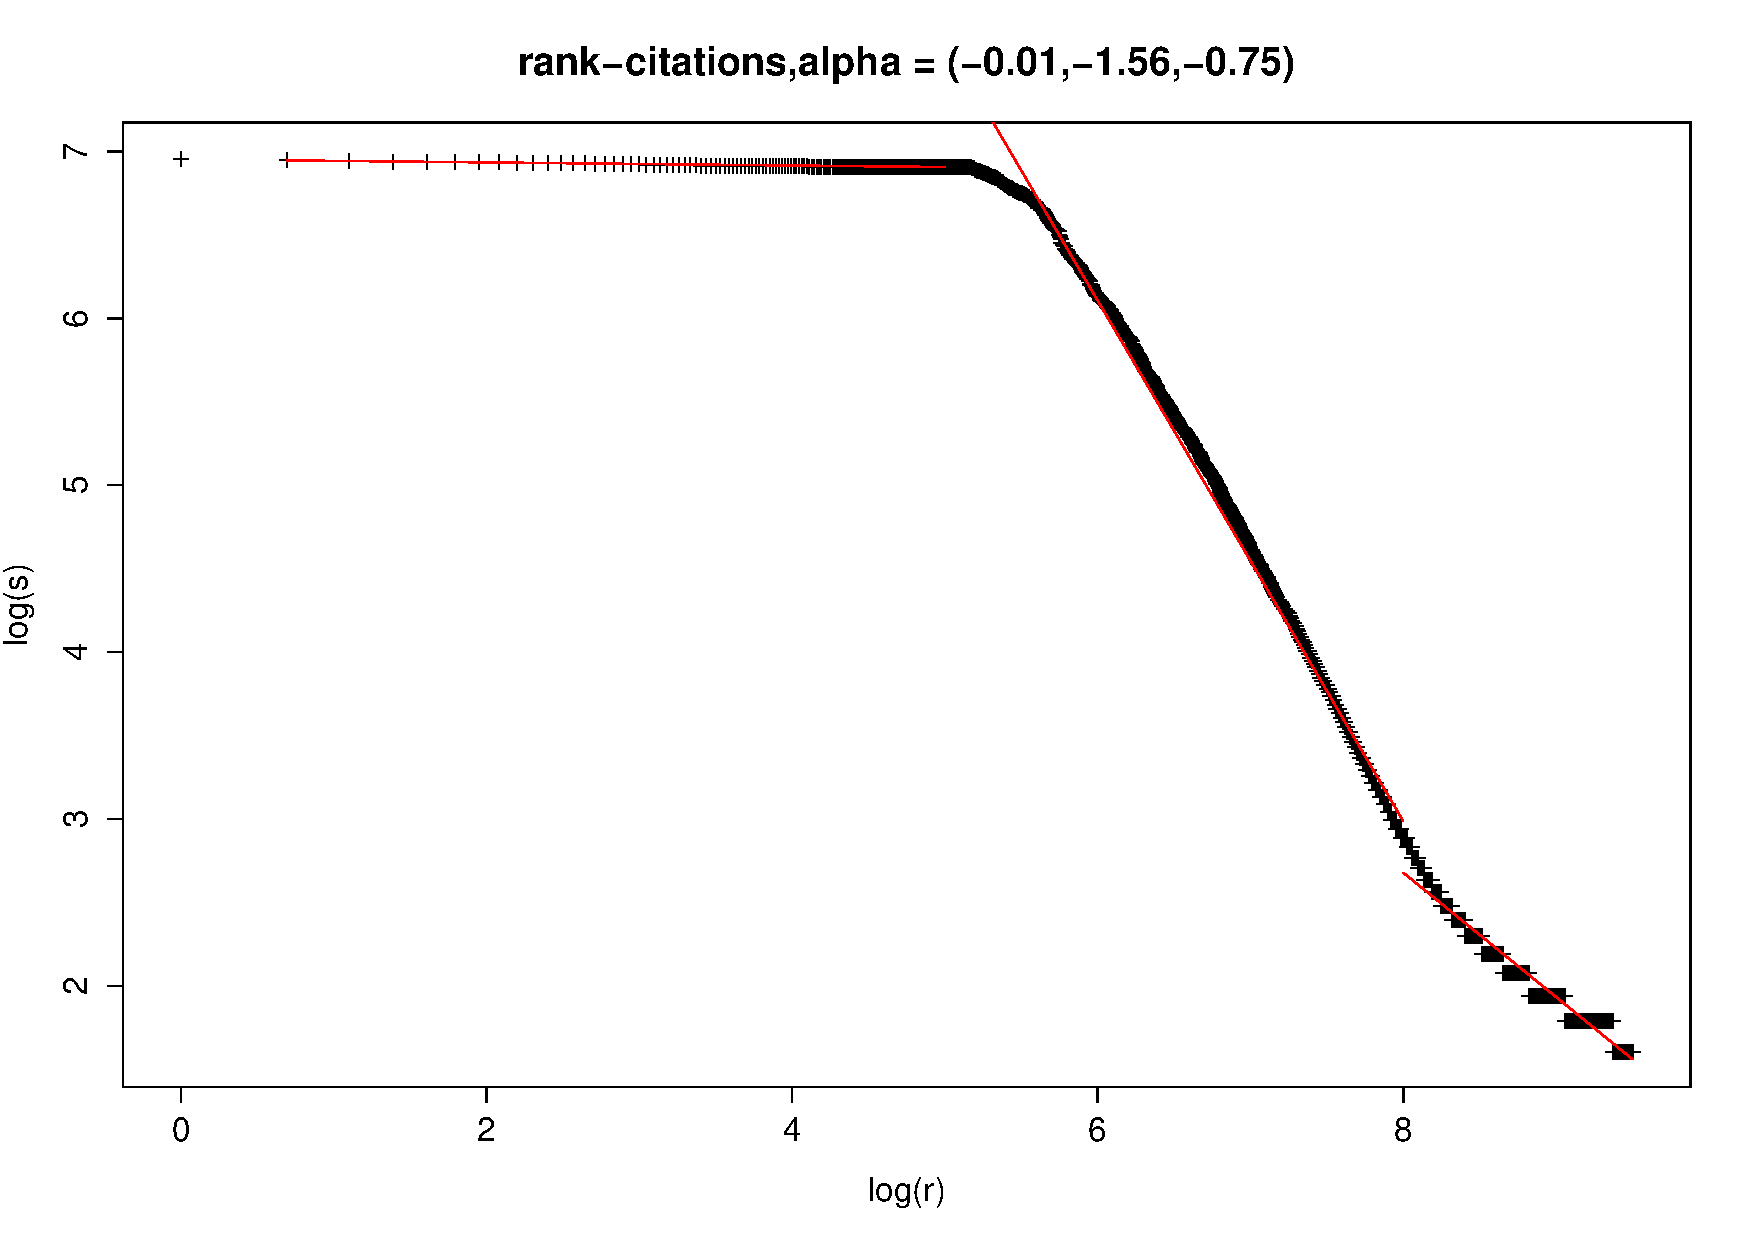
\includegraphics[width=\textwidth]{figures/rank-size-all}
%\hspace{-3cm}
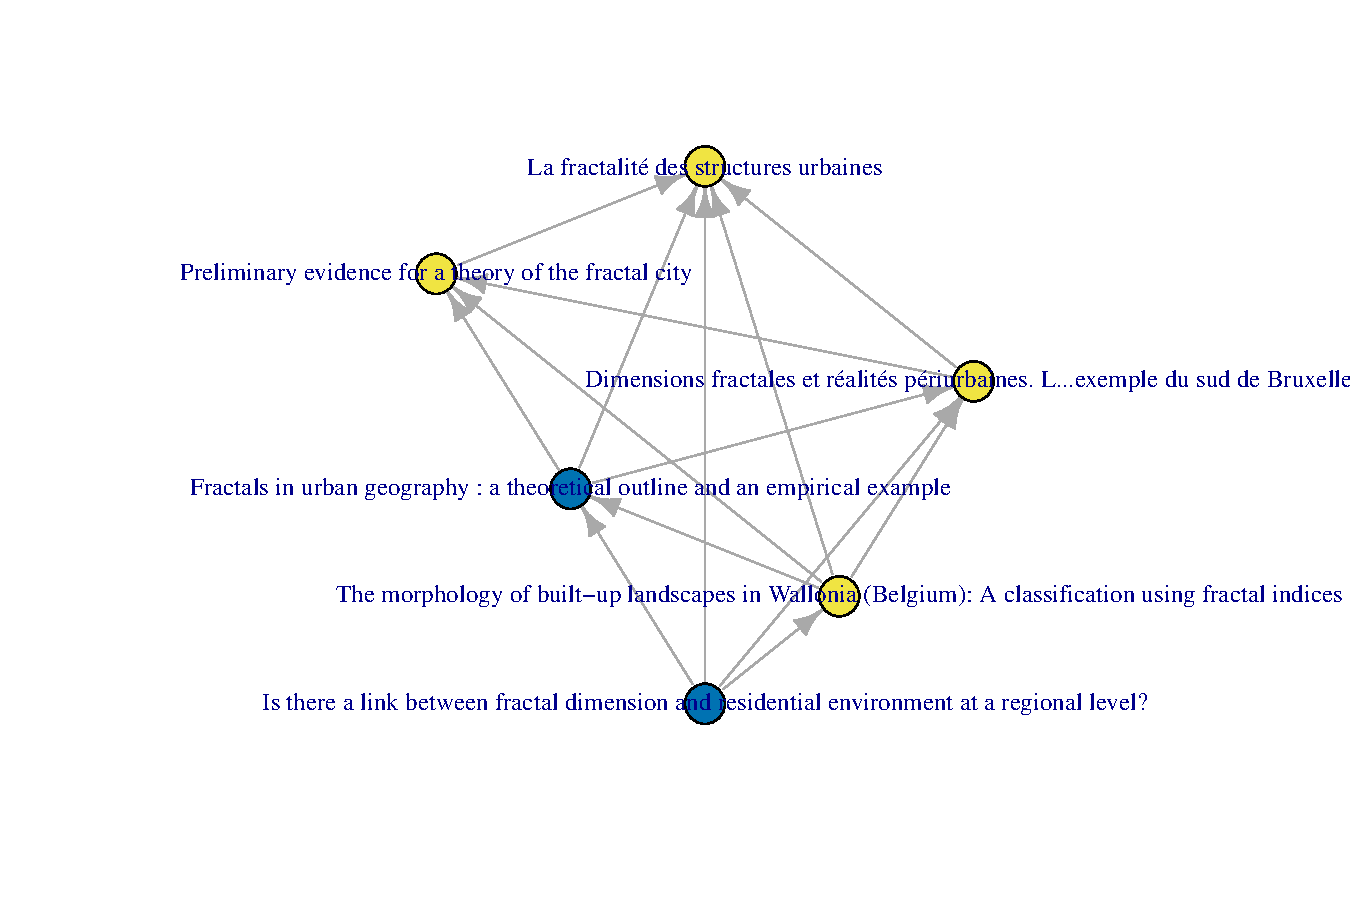
\includegraphics[width=\textwidth]{figures/cybclic_2cyb_13761}
\caption[Properties of the citation network]{Properties of the citation network. Top : Rank-size plot of in-degrees ; three superposing successive regimes must correspond to different literature types or practices across disciplines. Bottom : example of a maximal clique in the citation network, paper of \texttt{cybergeo} being in blue.}
\label{fig:quantepistemo:citnw}
\end{figure}
%%%%%%%%%%%%%%%%%


%%%%%%%%%%%%%%%%%%
\begin{figure}
\hspace{-2cm}
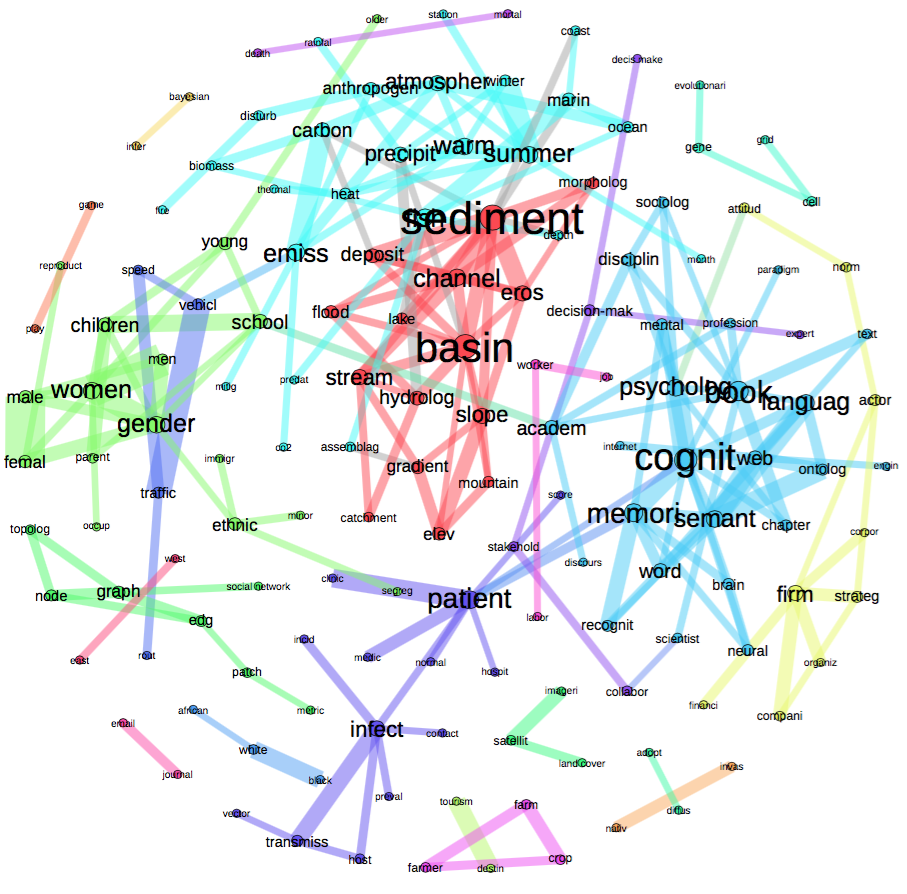
\includegraphics[width=1.4\textwidth]{figures/all_lesslinks}
\caption[Semantic network of concepts in quantitative geography]{Semantic network of concepts in quantitative geography. Corpus consists of around $2\cdot 10^5$ abstracts of publications at a topological distance shorter than 2 from the journal \texttt{cybergeo} in the citation network. Relevance of keywords were estimated with a bootstrap method, and semantic network is constructed by co-occurrences of keywords (cut at larger degrees, 10\% here to delete hubs such as \texttt{model} or \texttt{space} and efficiently reveal communities).}
\label{fig:quantepistemo:semanticnw}
\end{figure}
%%%%%%%%%%%%%%%%%%










%\begin{acknowledgements}
%If you'd like to thank anyone, place your comments here
%and remove the percent signs.
%\end{acknowledgements}

% BibTeX users please use one of
\bibliographystyle{spbasic}      % basic style, author-year citations
\bibliography{../Biblio/cybergeo}   % name your BibTeX data base







%%%%%%%%%%%%%%%%%%%%%
%%   Templates
%%%%%%%%%%%%%%%%%%%%%


%
%% For one-column wide figures use
%\begin{figure}
%% Use the relevant command to insert your figure file.
%% For example, with the graphicx package use
%  \includegraphics{example.eps}
%% figure caption is below the figure
%\caption{Please write your figure caption here}
%\label{fig:1}       % Give a unique label
%\end{figure}
%%
%% For two-column wide figures use
%\begin{figure*}
%% Use the relevant command to insert your figure file.
%% For example, with the graphicx package use
%  \includegraphics[width=0.75\textwidth]{example.eps}
%% figure caption is below the figure
%\caption{Please write your figure caption here}
%\label{fig:2}       % Give a unique label
%\end{figure*}
%%
%% For tables use
%\begin{table}
%% table caption is above the table
%\caption{Please write your table caption here}
%\label{tab:1}       % Give a unique label
%% For LaTeX tables use
%\begin{tabular}{lll}
%\hline\noalign{\smallskip}
%first & second & third  \\
%\noalign{\smallskip}\hline\noalign{\smallskip}
%number & number & number \\
%number & number & number \\
%\noalign{\smallskip}\hline
%\end{tabular}
%\end{table}
%











\end{document}
% end of file template.tex

